\documentclass[10pt,twocolumn,letterpaper]{article}

\usepackage{cvpr}
\usepackage{times}
\usepackage{epsfig}
\usepackage{graphicx}
\usepackage{epstopdf}
%\DeclareGraphicsExtensions{.eps}
\usepackage{amsmath}
\usepackage{amssymb}
\usepackage{lipsum}

% Include other packages here, before hyperref.

% If you comment hyperref and then uncomment it, you should delete
% egpaper.aux before re-running latex.  (Or just hit 'q' on the first latex
% run, let it finish, and you should be clear).
\usepackage[pagebackref=true,breaklinks=true,letterpaper=true,colorlinks,bookmarks=false]{hyperref}

% \cvprfinalcopy % *** Uncomment this line for the final submission

\def\cvprPaperID{[Scene Flow Estimation]} % *** Enter the CVPR Paper ID here
\def\httilde{\mbox{\tt\raisebox{-.5ex}{\symbol{126}}}}

% Pages are numbered in submission mode, and unnumbered in camera-ready
\ifcvprfinal\pagestyle{empty}\fi
\begin{document}

%%%%%%%%% TITLE
\title{\LaTeX\ Author Guidelines for CVPR Proceedings}

\author{
Hongyuan Ji\\
University of Michigan\\
{\tt\small hongyji@umich.edu}
\and
Jonathan Kurzer\\
University of Michigan\\
{\tt\small kurzerjo@umich.edu}
}

\maketitle
%\thispagestyle{empty}

%%%%%%%%% ABSTRACT
\begin{abstract}
   Briefly summarize the common topic of the three papers chosen and how each contributes to the field.
\end{abstract}

%%%%%%%%% BODY TEXT
\section{Paper Critiques}
\lipsum[1]

%-------------------------------------------------------------------------
\subsection{Non-Local Total Generalized Variation for Optical Flow Estimation ~\cite{ranftl2014non}}

\subsubsection{Problem Statement}
\lipsum[1]

\subsubsection{Innovation or claim}
\lipsum[1]

\subsubsection{How is the innovation done or what is the mathematical model}
\lipsum[1]

\subsubsection{How is the innovation evaluated}
\lipsum[1]

\subsubsection{Did the innovation substantiate the claim to solve the problem}
\lipsum[1]

%-------------------------------------------------------------------------
\subsection{Dense Trajectories and Motion Boundary Descriptors for Action Recognition ~\cite{wang2013dense}}

\subsubsection{Problem Statement}
\lipsum[1]

\subsubsection{Innovation or claim}
\lipsum[1]

\subsubsection{How is the innovation done or what is the mathematical model}
\lipsum[1]

\subsubsection{How is the innovation evaluated}
\lipsum[1]

\subsubsection{Did the innovation substantiate the claim to solve the problem}
\lipsum[1]

%-------------------------------------------------------------------------
\subsection{A Quantitative Analysis of Current Practices in Optical Flow Estimation and the Principles Behind Them ~\cite{sun2014quantitative}}

\subsubsection{Problem Statement}
\lipsum[1]

\subsubsection{Innovation or claim}
\lipsum[1]

\subsubsection{How is the innovation done or what is the mathematical model}
\lipsum[1]

\subsubsection{How is the innovation evaluated}
\lipsum[1]

\subsubsection{Did the innovation substantiate the claim to solve the problem}
\lipsum[1]

%------------------------------------------------------------------------
\section{Implementation}
\begin{equation}
E(\textbf{u}) = E_D(\textbf{u}) + \lambda_l E_L(\textbf{u})
+ \lambda_n \underbrace{\sum_i \sum_{j>i} \omega_{ij} \rho_N(u_i-u_j)}_{E_N(\textbf{u})}
\end{equation}
\begin{equation}
\omega_{ij} = k(\textbf{f}_i,\textbf{f}_i) = 
\text{exp}\left(-\frac{||\textbf{p}_i-\textbf{p}_j||^2}{2 \sigma^2_x}
- \frac{||\textbf{c}_i-\textbf{c}_j||^2}{2 \sigma^2_c}\right)
\end{equation}
\begin{equation}
q_i = \sum_j A_{ij} p_j = p_i \sum_j k(\textbf{f}_i,\textbf{f}_j)
- \sum_j k(\textbf{f}_i,\textbf{f}_j) p_j
\end{equation}
\begin{equation}
\rho(x) \approx \mu_{\omega,\sigma}(x) = T - \sum^K_{n=1} \omega_n \text{ exp}\left(-\frac{x^2}{2\sigma^2_n}\right)
\end{equation}
\begin{figure}[t]
\begin{center}
   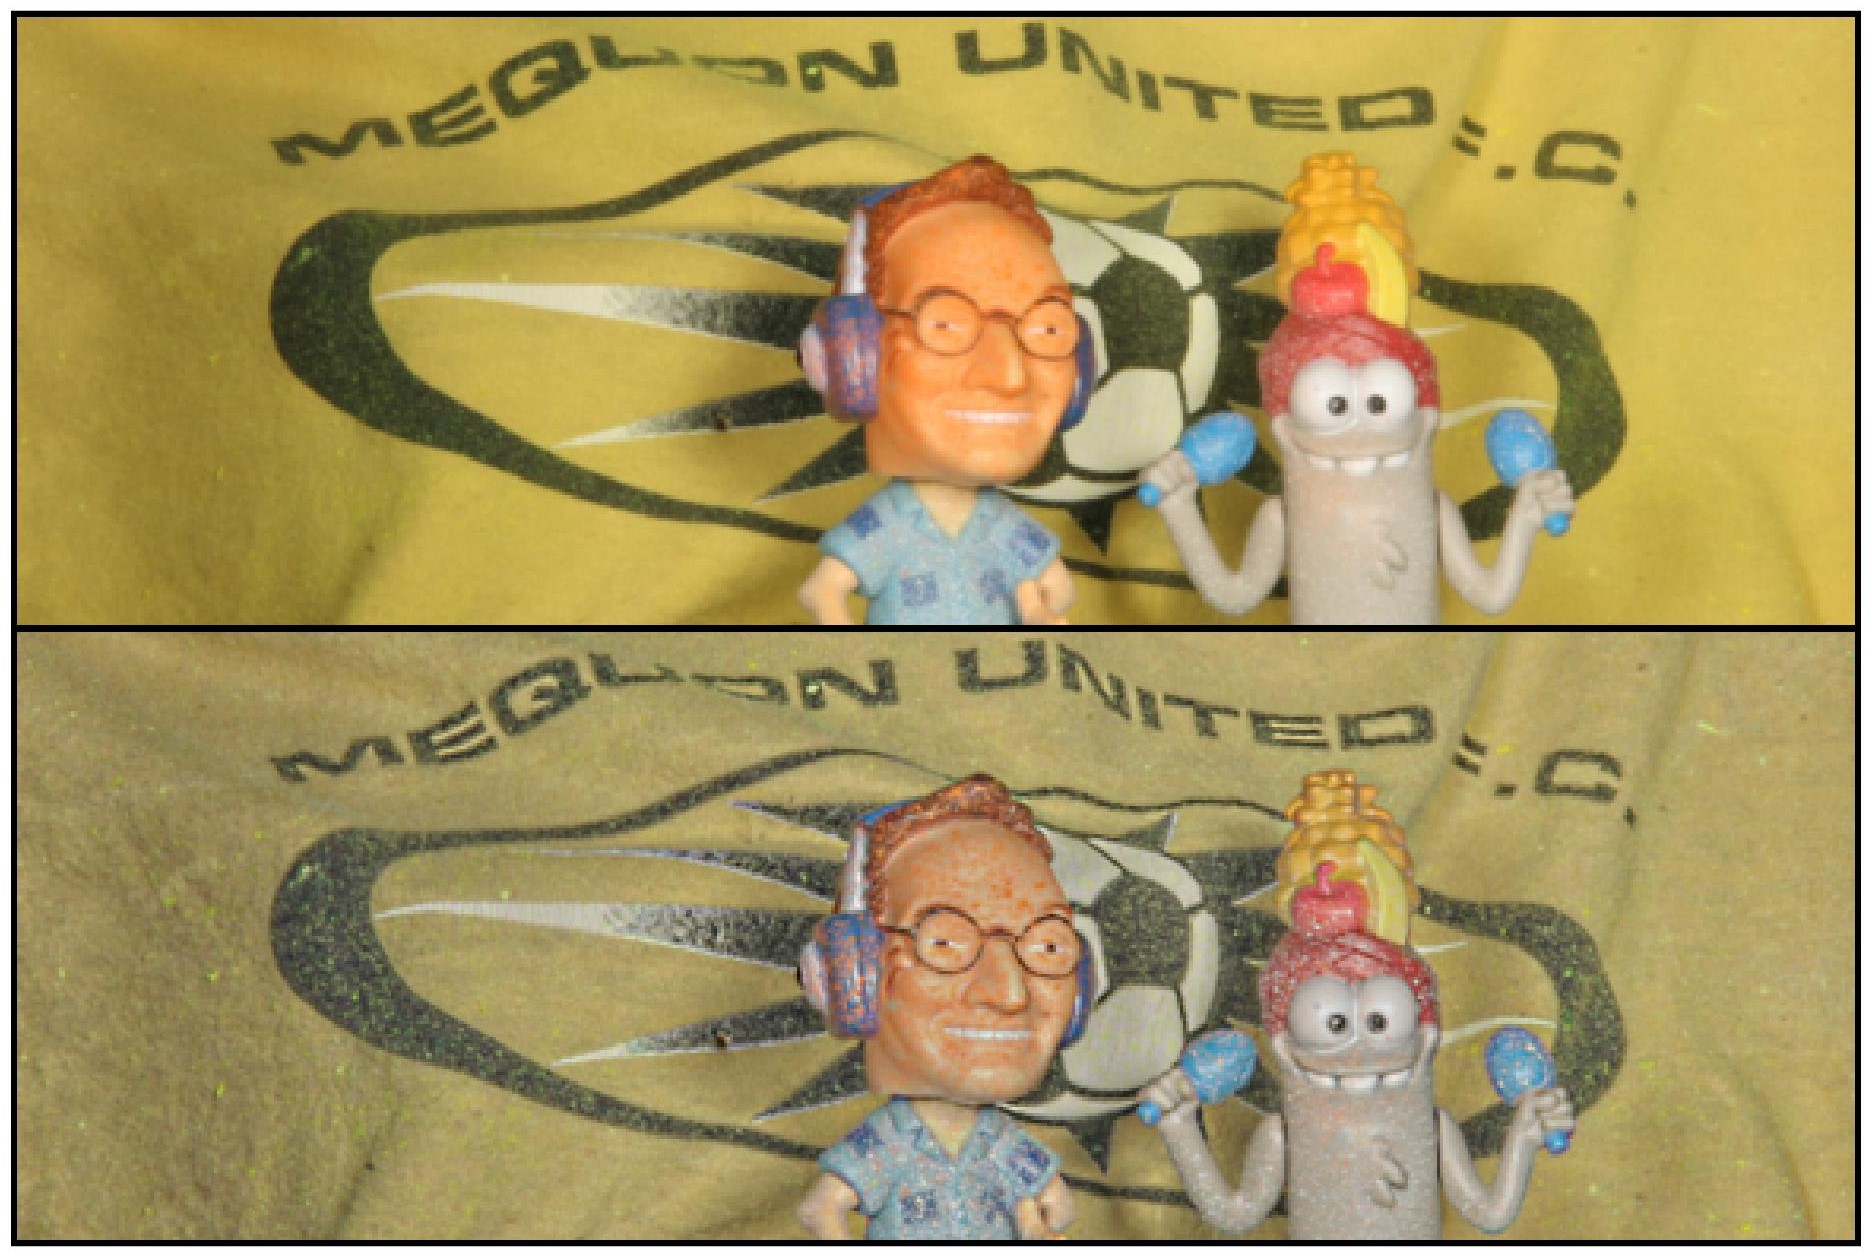
\includegraphics[width=.8\linewidth]{figs/structureDecomp.jpg}
\end{center}
   \caption{TODO TODO TODO TODO}
\label{fig:structure}
\end{figure}

\begin{figure}[t]
\begin{center}
   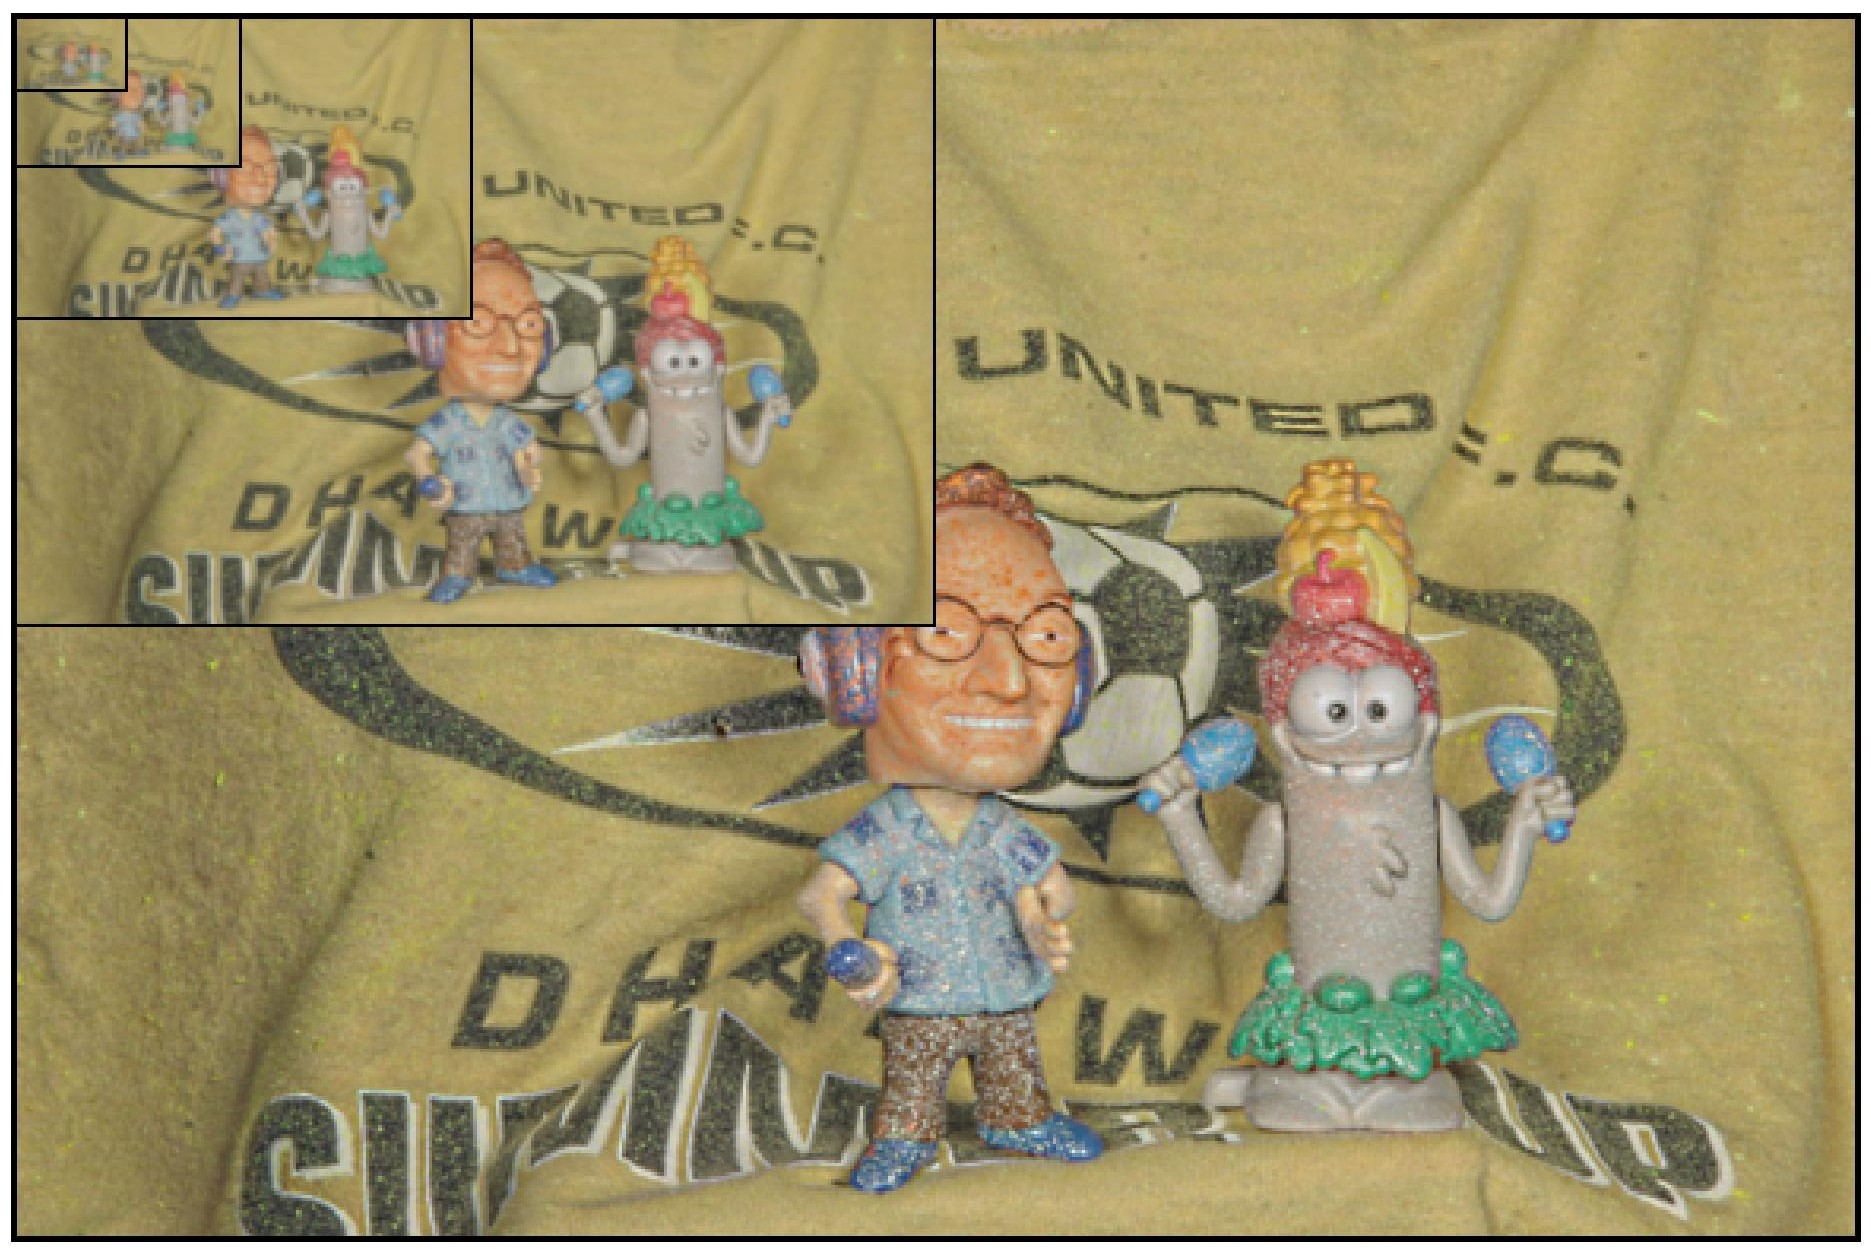
\includegraphics[width=.8\linewidth]{figs/pyramids.jpg}
\end{center}
   \caption{TODO TODO TODO TODO}
\label{fig:structure}
\end{figure}

\begin{figure}[t]
\begin{center}
   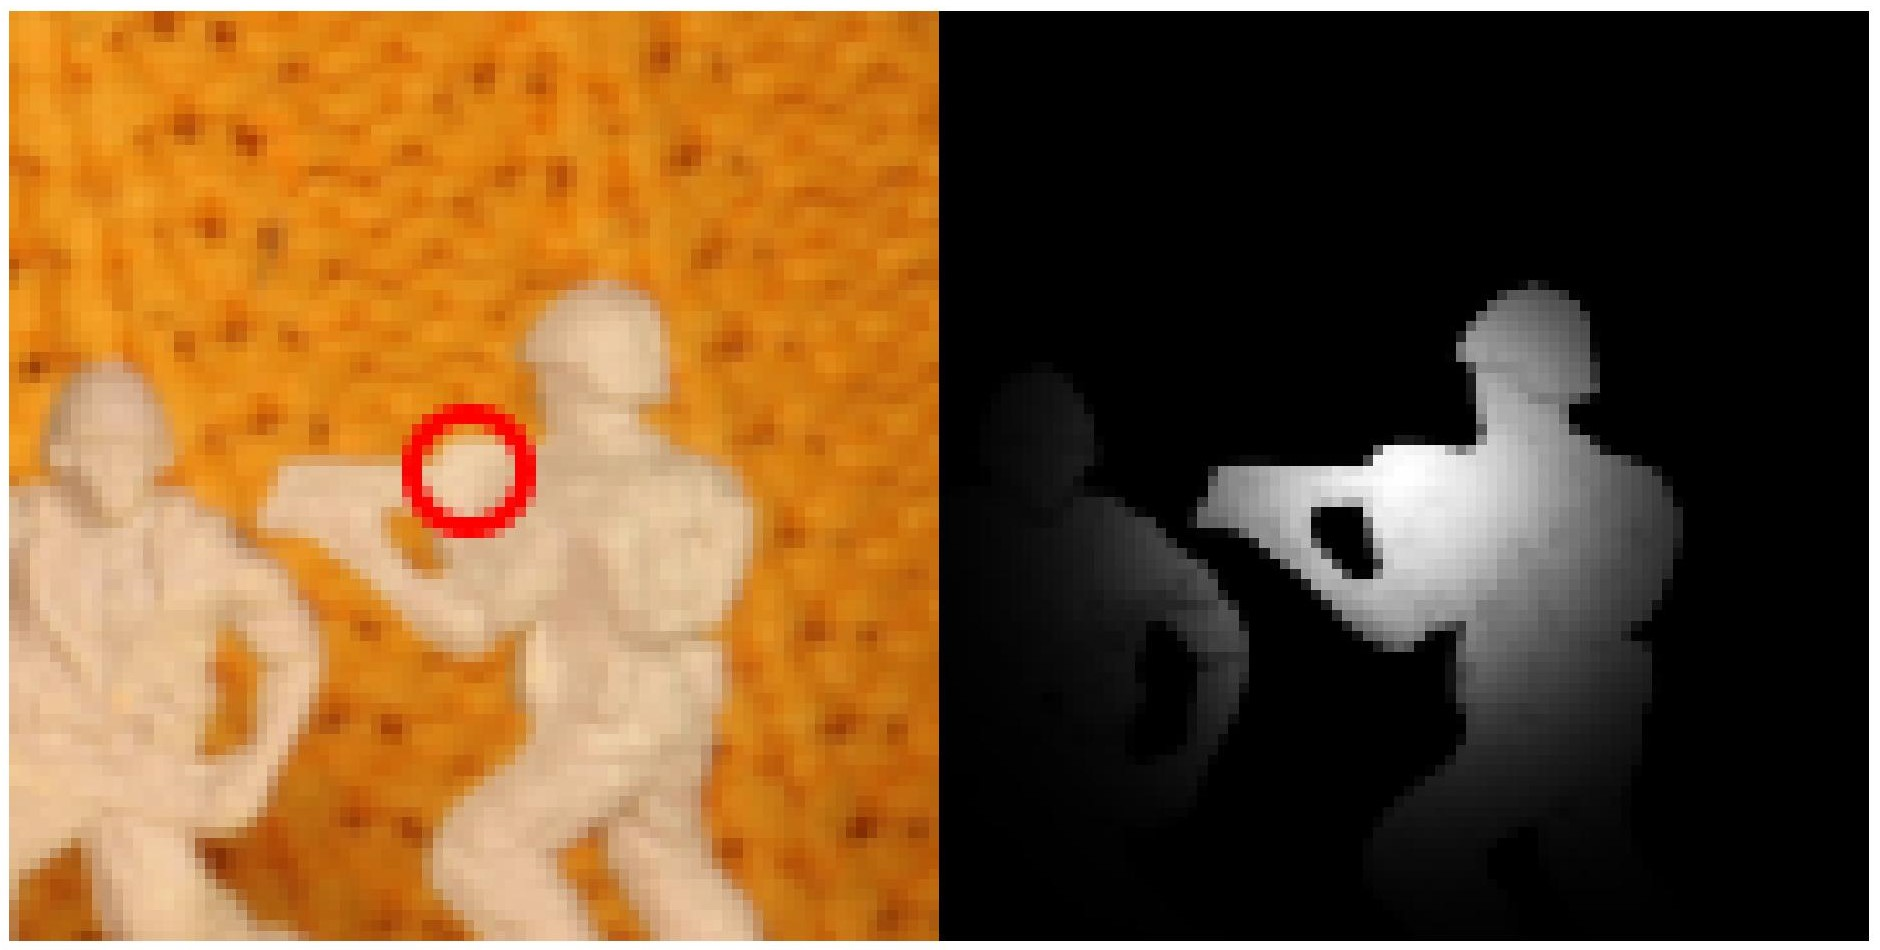
\includegraphics[width=.8\linewidth]{figs/nonLocalWieght.jpg}
\end{center}
   \caption{TODO TODO TODO TODO}
\label{fig:structure}
\end{figure}

\begin{figure}[t]
\begin{center}
   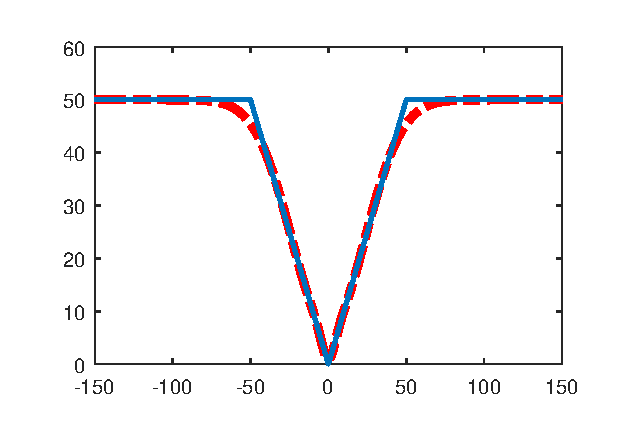
\includegraphics[width=0.8\linewidth]{figs/penalty_l1Norm.eps}
\end{center}
   \caption{TODO TODO TODO TODO}
\label{fig:structure}
\end{figure}

\begin{figure}[t]
\begin{center}
   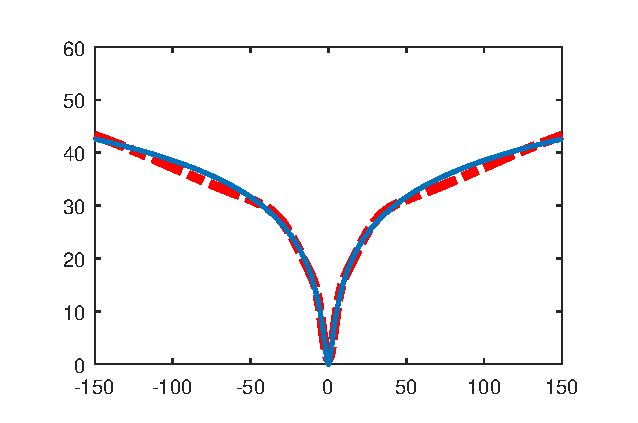
\includegraphics[width=0.8\linewidth]{figs/penalty_Lorentzian.eps}
\end{center}
   \caption{TODO TODO TODO TODO}
\label{fig:structure}
\end{figure}

\begin{figure}[t]
\begin{center}
   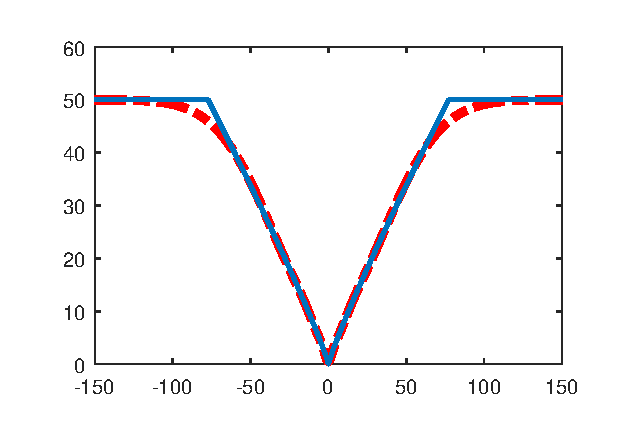
\includegraphics[width=0.8\linewidth]{figs/penalty_GenCharbonnier.eps}
\end{center}
   \caption{TODO TODO TODO TODO}
\label{fig:structure}
\end{figure}


\lipsum

{\small
\bibliographystyle{ieee} 
\bibliography{egbib}
}

\end{document}
